\section{Question I: Revisiting HW4 Bank Classification with New Tools (for dataset A)}
\subsection{Data preprocessing}
For this part of the assignment, the dataset had to be analyzed first as part of the preprocessing step to get the structure, detect issues such as missing values and find outliers. The bank marketing data (bank-additional.csv) has 4119 observations and 21 features. There was found to be 1230 unknowns in the categorical features of the dataset. Features that had unknowns were checked and there was found to be six features: job, marital, education, default, housing, and  loan that had unknowns (0.96\% , 0.3\% , 4.1\%, 19.5\%, 2.6\%, 2.6\%) respectively. Removing rows with missing values can be too limiting on some predictive modeling problems. Although the default  column was dropped because it has 803 missing values accounting for almost 20\% of the feature. For the other 5 features the proportion of the unknown's is sparse, the mode of the categorical features was used to replace the unknown's. Also, the "duration" feature was dropped since this attribute highly affects the output target (e.g., if duration=0 then y='no').

The categorical predictor variables  were converted  to numerical using the "get\_dummies" function ,appending the structure to 48 features (4119,48).
The "pdays" feature was particularly challenging to deal with because of the massive variation in the values. Many of the samples had a "pdays" value of 999 indicating that the person was never contacted. We felt it would be better to represent this feature as a set of labels corresponding to how recent the person was contacted. The pandas function "pandas.cut" was used to perform this transformation and results in four bins (less than 1 week, less than 2 weeks, less than 1 month and never).

Finally the numerical features were explored for inconsistencies and outliers. A series of box plots were used to visualize the spread of the numerical data as seen in Figure~\ref{fig:fig1} below. None of the numerical features had outliers or skews that would cause concern.
\begin{figure}[h!]
  \centering
  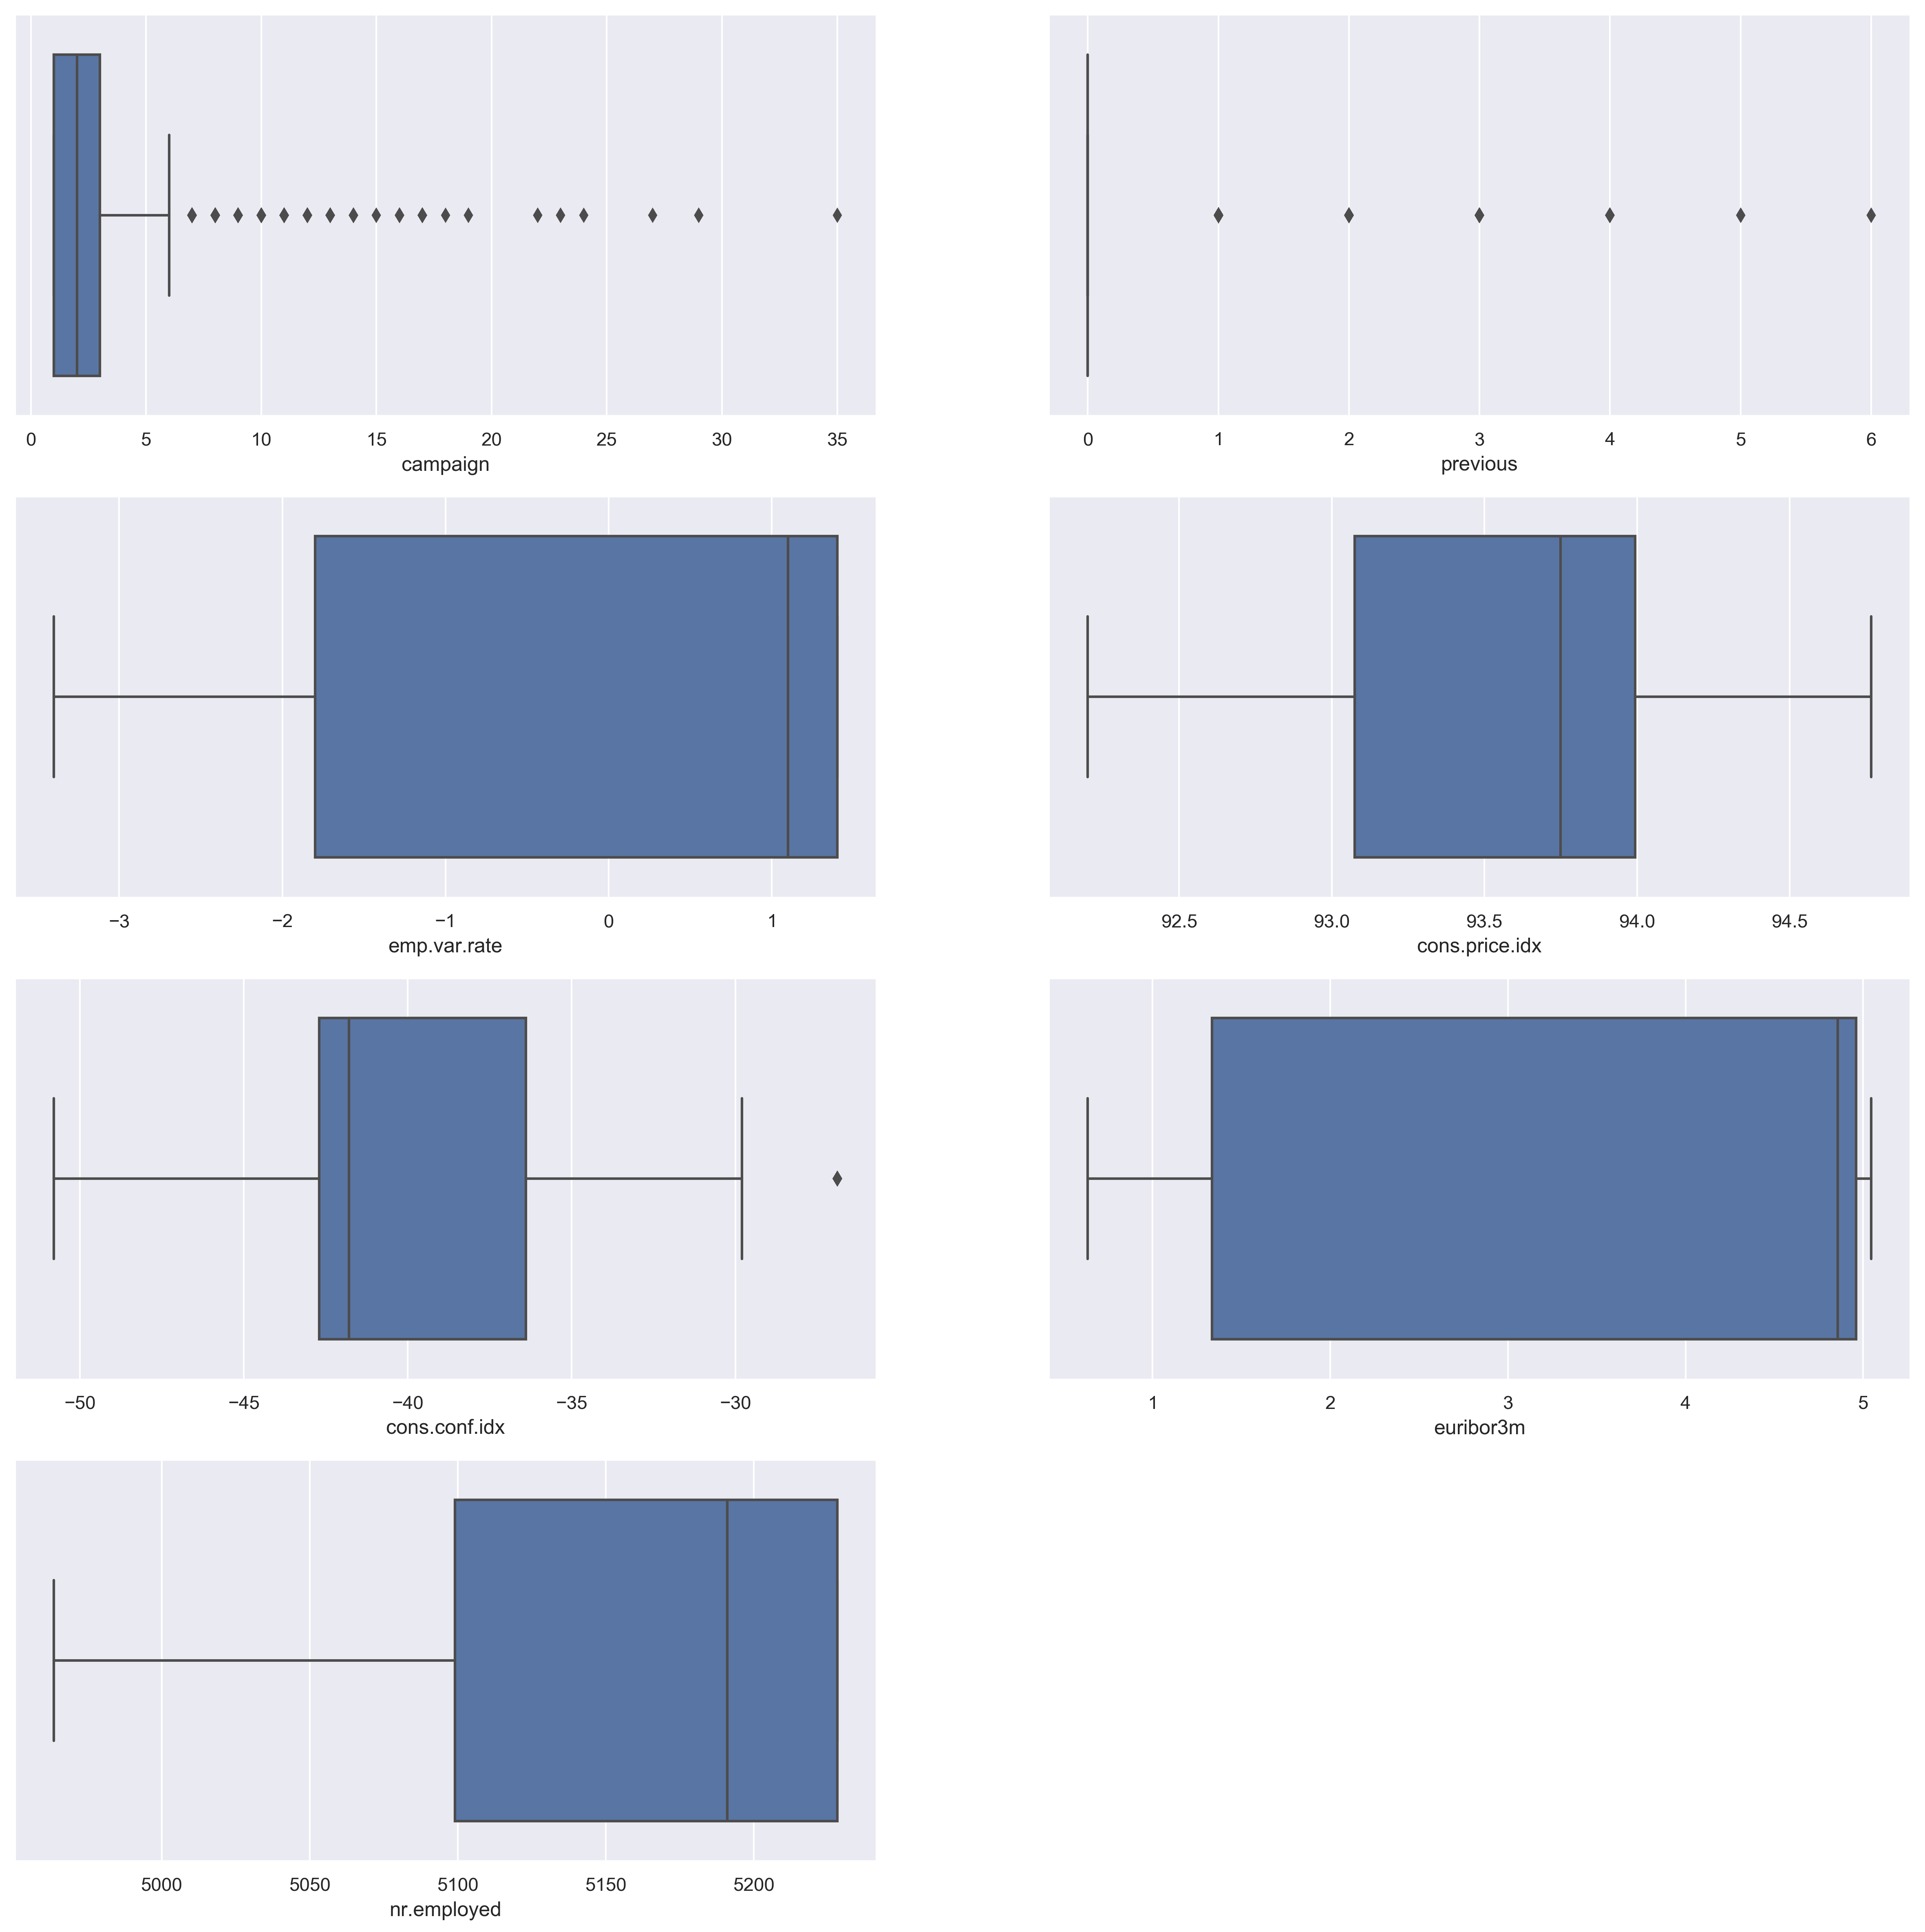
\includegraphics[width=4.1in]{assignment2/1-1-boxplots.png}
  \caption{Boxplot to detect outliers}
  \label{fig:fig1}
\end{figure}

\newpage
\subsection{Dividing data into training and testing}
For dividing the data-set(4119 samples), 80\% was used for training and 20\% for testing. This split was chosen after researching best practices for splitting data\cite{ref_article1}. Splitting the data is important to allow validation of the trained models and detect common problems, such as over fitting. Certain algorithms are impacted more from over fitting than others. Neural networks and support vector machines are more sensitive to over fitting, however, algorithms such as Naive Bayes are generally more resilient to the problem.

A decision or argument could be made to increase the fraction of the test split as this would give more values to validate over, however this comes at the cost of having less data to train the initial model. Due to this trade off we decided that 80/20 gives a decent balance of data to train and samples to validate against.


\subsection{Applying classification}


\subsubsection{Decision Tree (DT)}
The Depth of the tree was chosen as 3 for which the model performed more accurately without over-fitting. We first plotted the area under curve score (AUC score) against the tree depth (figure 1 below).
\begin{figure}[!ht]
 \centering
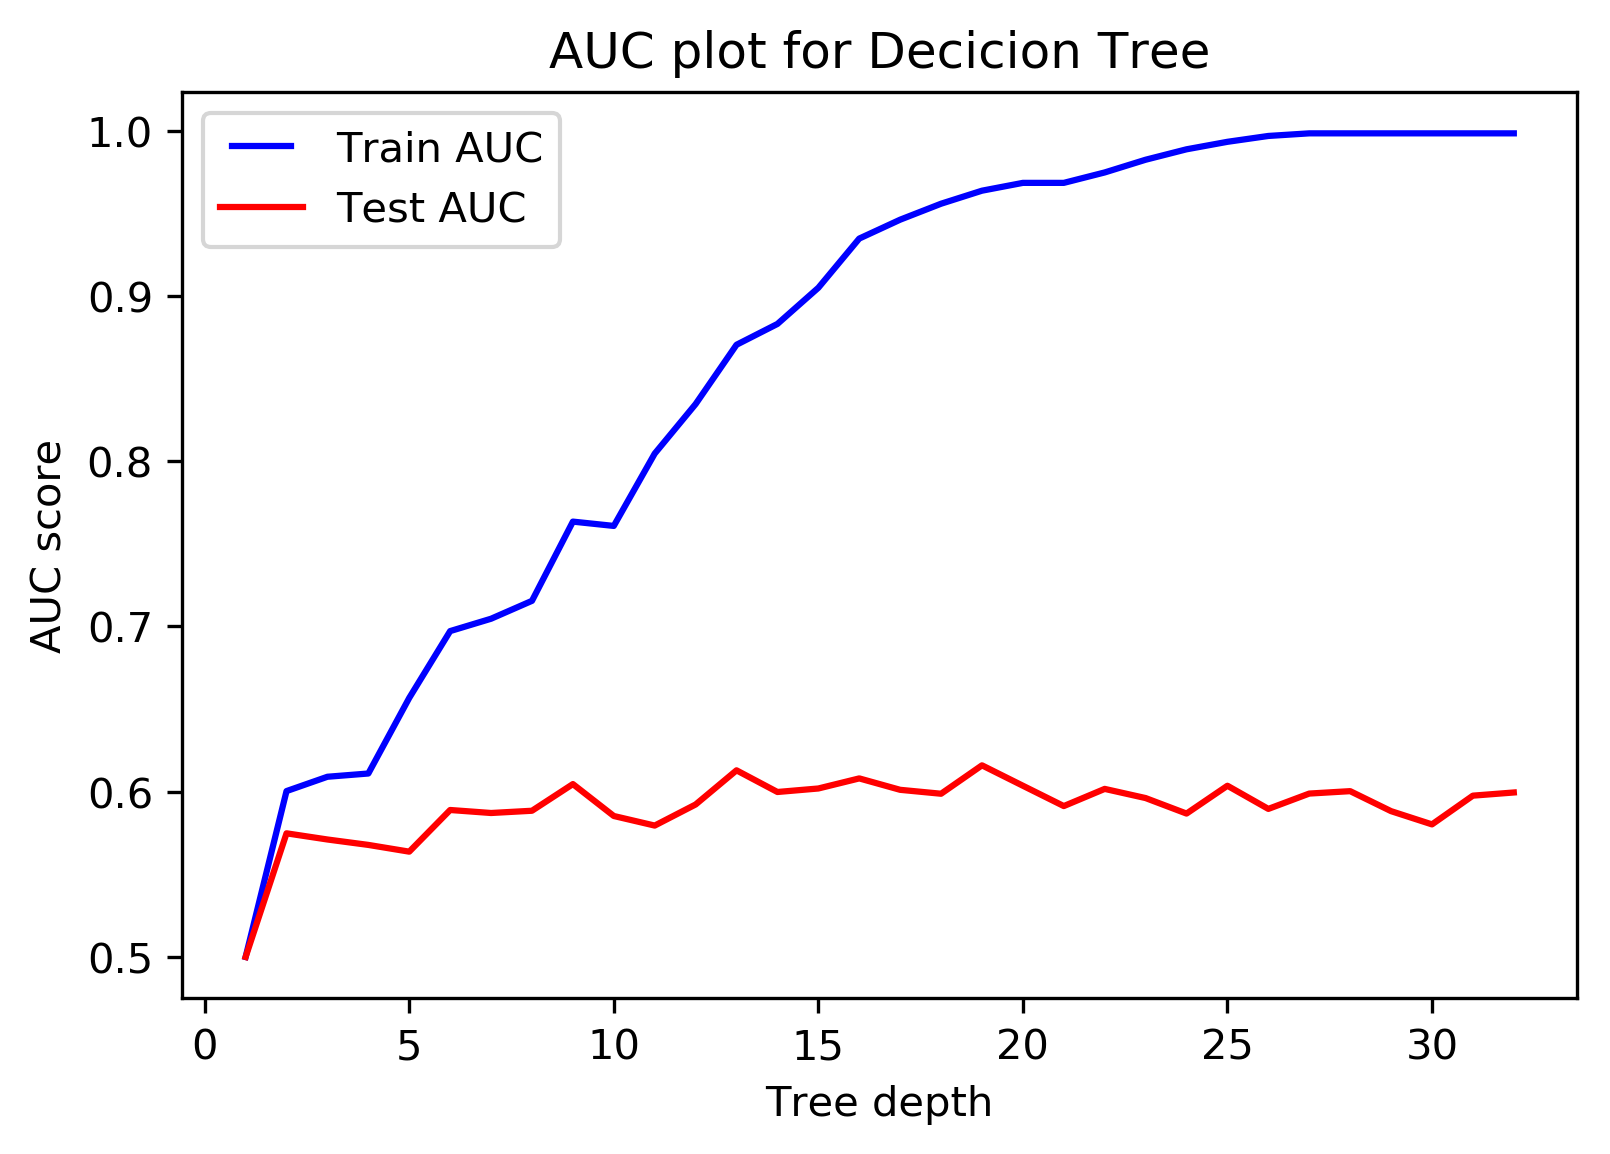
\includegraphics[width=3.1in]{assignment2/1-3-DecisionTree_AUC.png}
\caption{\label{fig:fig1}AUC score curve against tree depth}
\end{figure}
As it can be seen from the curve, the deeper the tree the higher the train AUC score but the test AUC score wont change a lot after tree depth of 3. This means that we get an overfitting case as our model will have a high AUC score (predicts the train data perfectly) for deeper tree depth but will fail to generalize and predict the test data. For this reason the tree depth was chose to be 3 for our model.
If the depth of tree was not specified, by default, scikit-learn will keep expanding the nodes until all the leaves contain less than min\_samples\_split samples and as we saw in the graph below, the higher value of maximum depth causes over-fitting, and a lower value causes under-fitting\cite{ref_url1}.

% ID3, or Iternative Dichotomizer, was the first of three Decision Tree implementations developed by Ross Quinlan
% It builds a decision tree for the given data in a top-down fashion, starting from a set of objects and a specification of properties Resources and Information. each node of the tree, one property is tested based on maximizing information gain and minimizing entropy, and the results are used to split the object set. This process is recursively done until the set in a given sub-tree is homogeneous (i.e. it contains objects belonging to the same category). The ID3 algorithm uses a greedy search. It selects a test using the information gain criterion, and then never explores the possibility of alternate choices.



According to scikit documentation, they uses an optimized version of the CART algorithm for the decision tree. CART stands for Classification and Regression Trees. It is characterized by the fact that it constructs binary trees, namely each internal node has exactly two outgoing edges. The splits are selected using the twoing criteria and the obtained tree is pruned by cost–complexity Pruning. CART can handle both numeric and categorical variables and it can easily handle outliers\cite{ref_url3}.
\\

\subsubsection{Random Forests (RF)}
The random forests classifier was built using the scikit-learn. The two main parameters that were considered here are the n\_estimator and tree depth. The n\_estimator simply represents the number of trees in the model and tree depth is the depth of those trees. Similar to the approach described in the decision tree, AUC score was plotted against n\_estimator and tree depth to observe any over-fitting cases. Figure~\ref{fig:fig2} shows the AUC scores for n\_estimator and figure~\ref{fig:fig3} shows the AUC scores for tree depth. Based on these graphs, the n\estimator was chosen to be as 16 and the depth of the tree as 3.
\begin{figure}[!ht]
 \centering
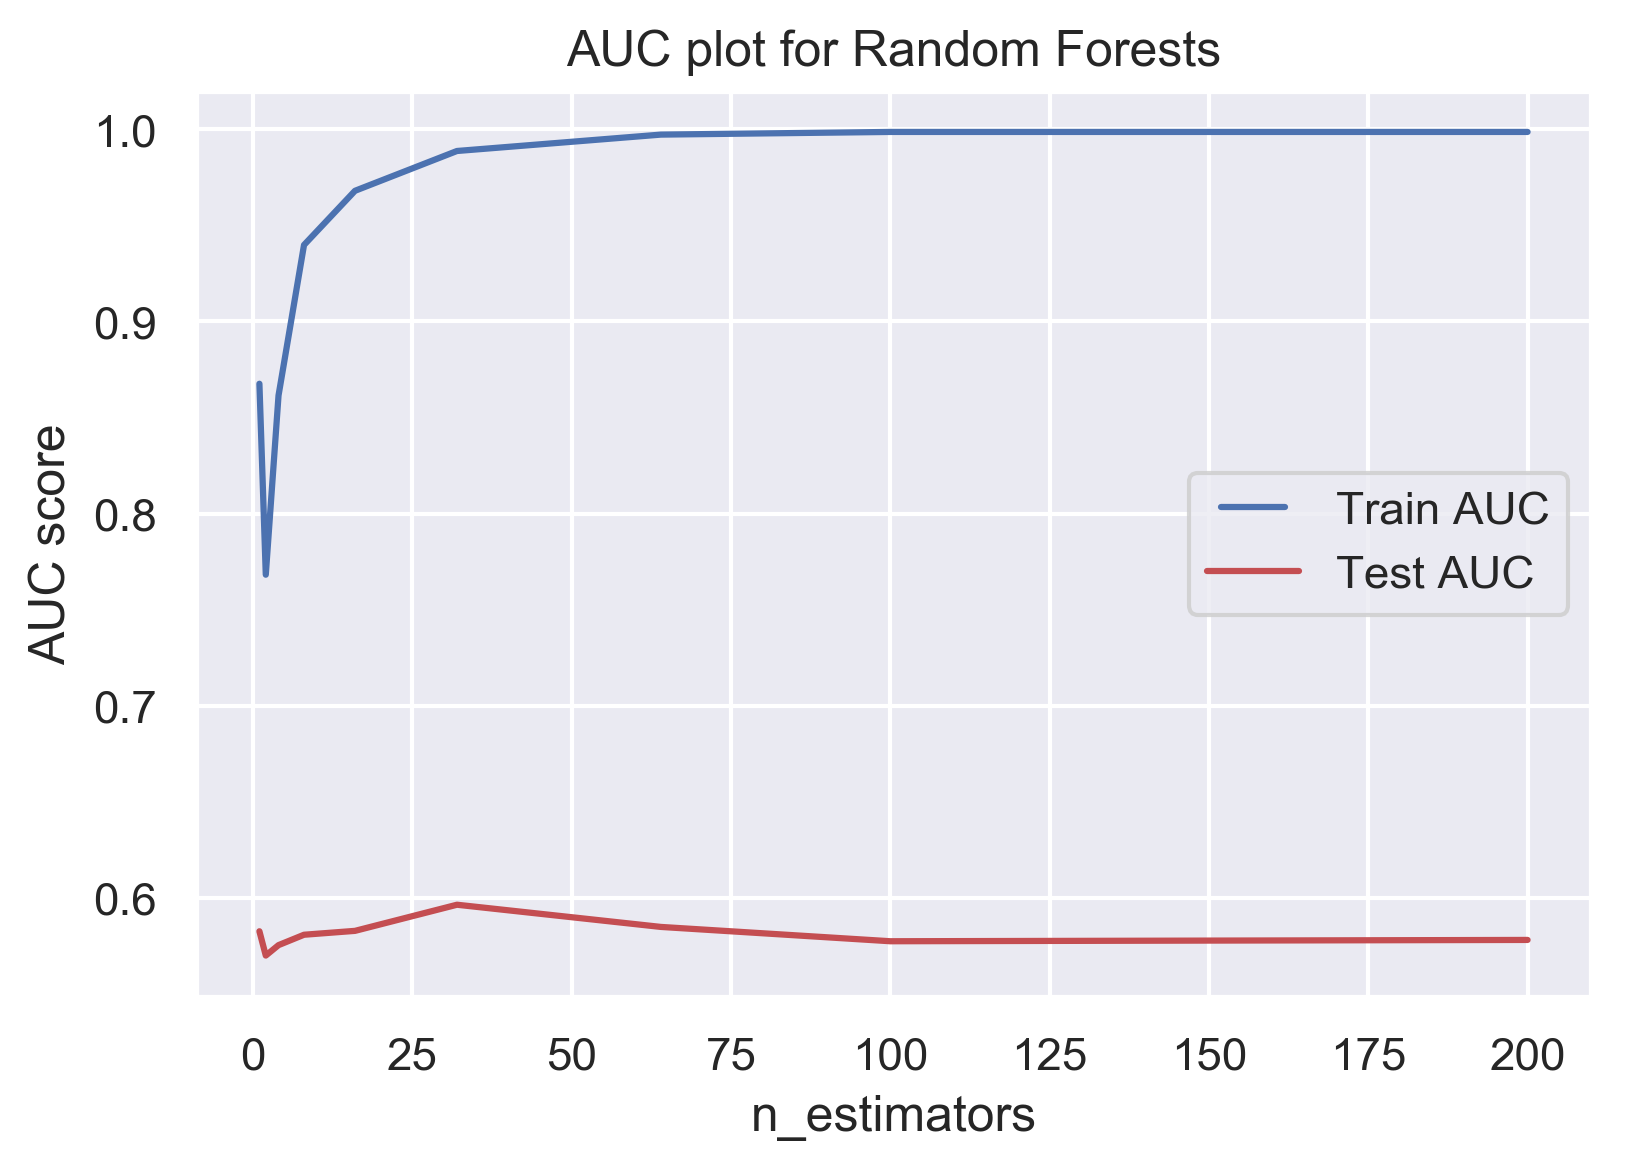
\includegraphics[width=3.1in]{assignment2/1-3-RandomForests_AUC(n_estimators).png}
\caption{\label{fig:fig2}AUC score curve against n\_estimators}
\end{figure}

\begin{figure}[!ht]
 \centering
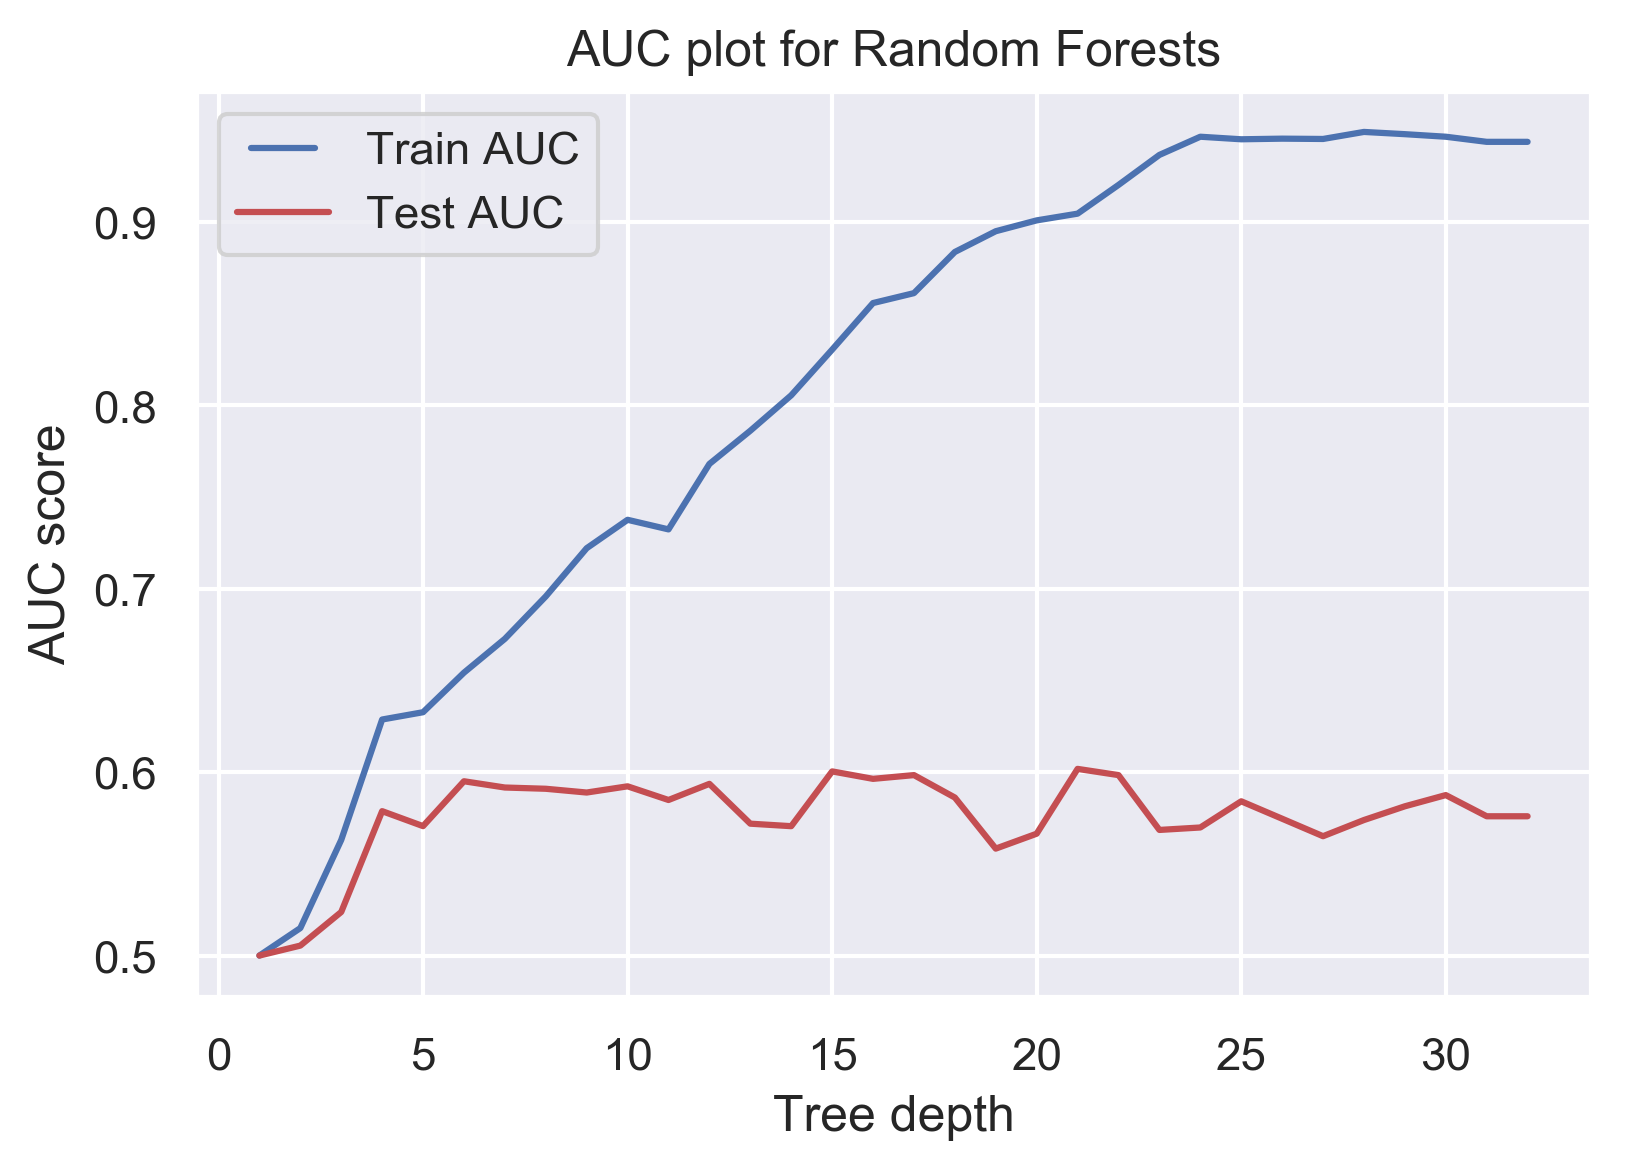
\includegraphics[width=3.1in]{assignment2/1-3-RandomForests_AUC(TreeDepth).png}
\caption{\label{fig:fig3}AUC score curve against tree depth}
\end{figure}

\\

\subsubsection{Neural Network (NN)}
Neural netwrok is made up of three main layers: input, hidden, and output layers. In our case, the input layer is made up of 46 layers (number of input features) and the output layer has a single node (outputs either 1 or 0). The way the neural network model works is that it receives an inputs and multiply them by some weight which is then passed to an activation function to predict an output. Then the output is compared with y\_test label in which the weights will be adjusted accordingly. The process repeated until the maximum number of iterations reached. For building our model, we used gridsearch built-in function which returns the best hyper-parameters from the parameter space list provided. The hyper-parameters that were tested are:\\
1- hidden layer sizes : [(32,32), (20,20), (47,47)] \\
2- activation function: ['tanh', 'relu'] \\
3- solver: ['sgd', 'adam','lbfgs'] \\
4- alpha: [0.0001, 0.05] \\
then the gridsearch returned the parameters that best performed. However, one thing to note is that even though there is no rule of thumb for choosing the number of neurons in the hidden layers, it should not exceed the number of input layers (46 in this case) to avoid over-fitting problems. 
The best parameters were found to be as follow: activation=tanh, alpha=0.0001, hidden layers = (32, 32), and solver = Stochastic Gradient Descent (SGD). 

\\






\subsection{Create a few plots of your model on the test data, two of the data dimensions at a time,indicating the predicted elements of each class using different colors or shapes. You may need to try plotting various pairs of dimensions to see which provide some interesting result. Be sure to label your axis and legend. Why is separation better on some plots than others}


\clearpage{}
\begin{figure}[!ht]
 \centering
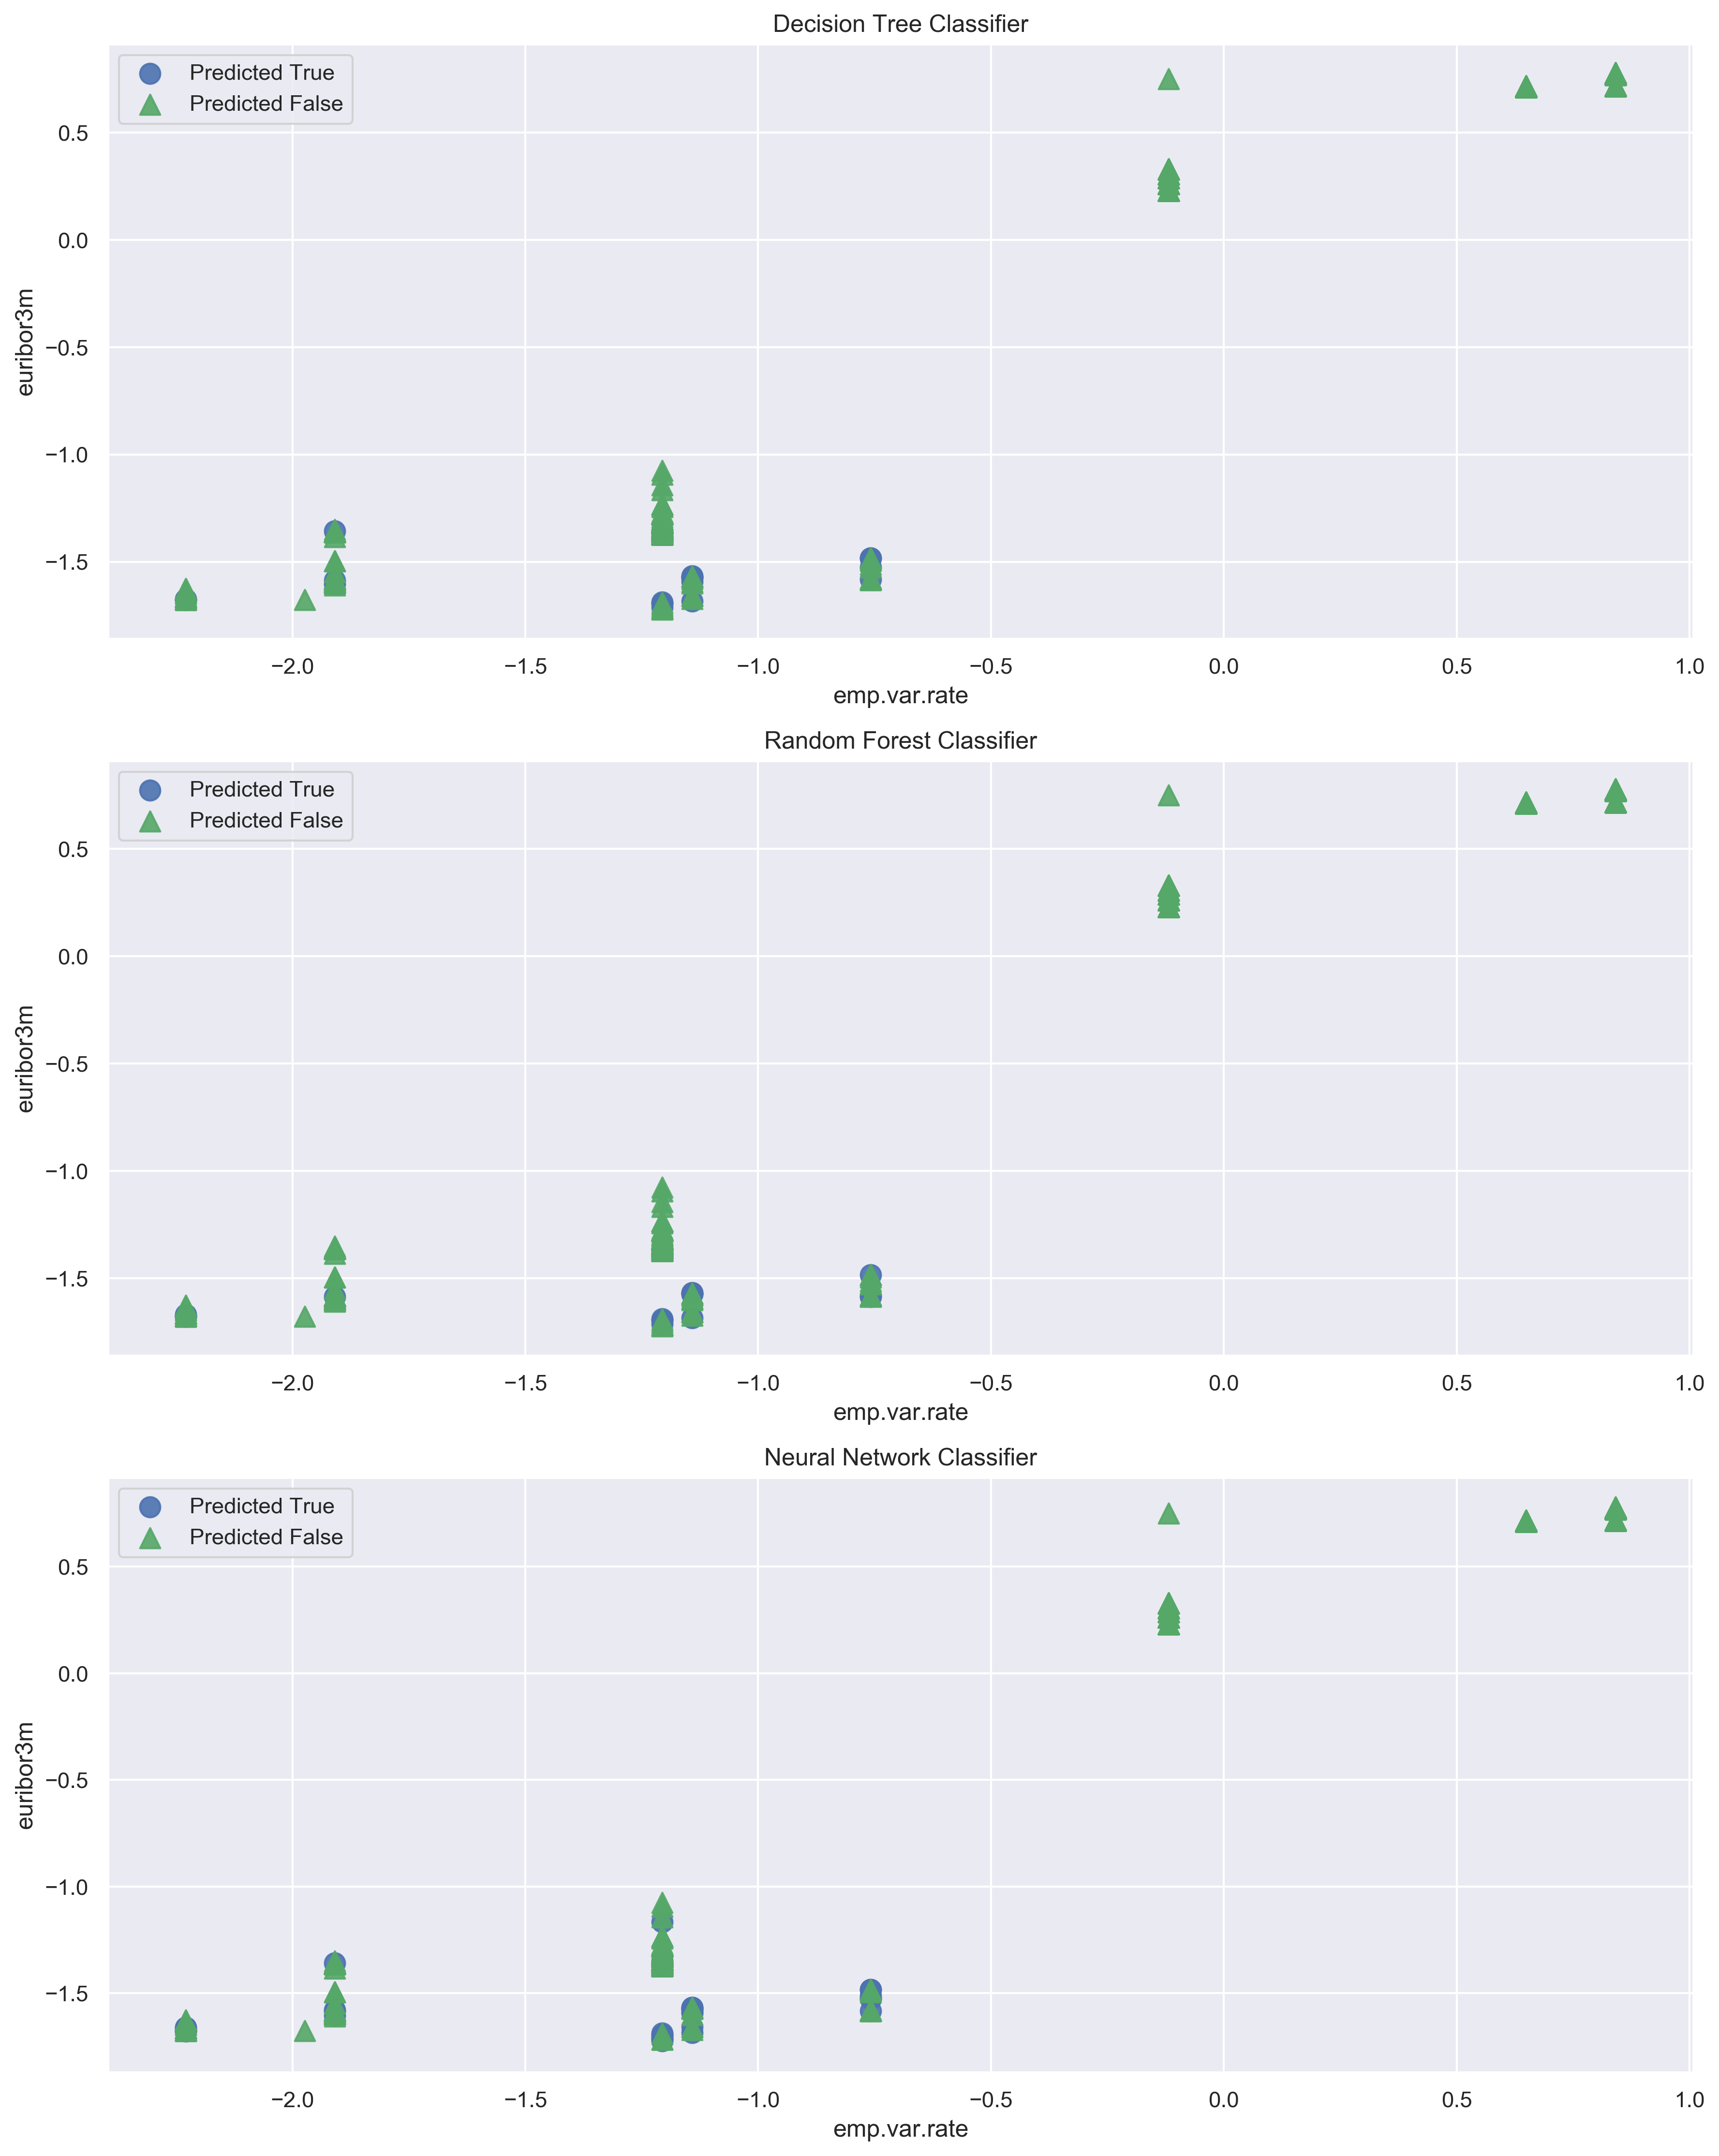
\includegraphics[width=2.5]{assignment2/1-4- eur and emp features.png}
\caption{\label{fig:2dplot1}Plot of euribor3m VS emp.var.rate }
\end{figure}



\clearpage{}
\begin{figure}[!ht]
 \centering
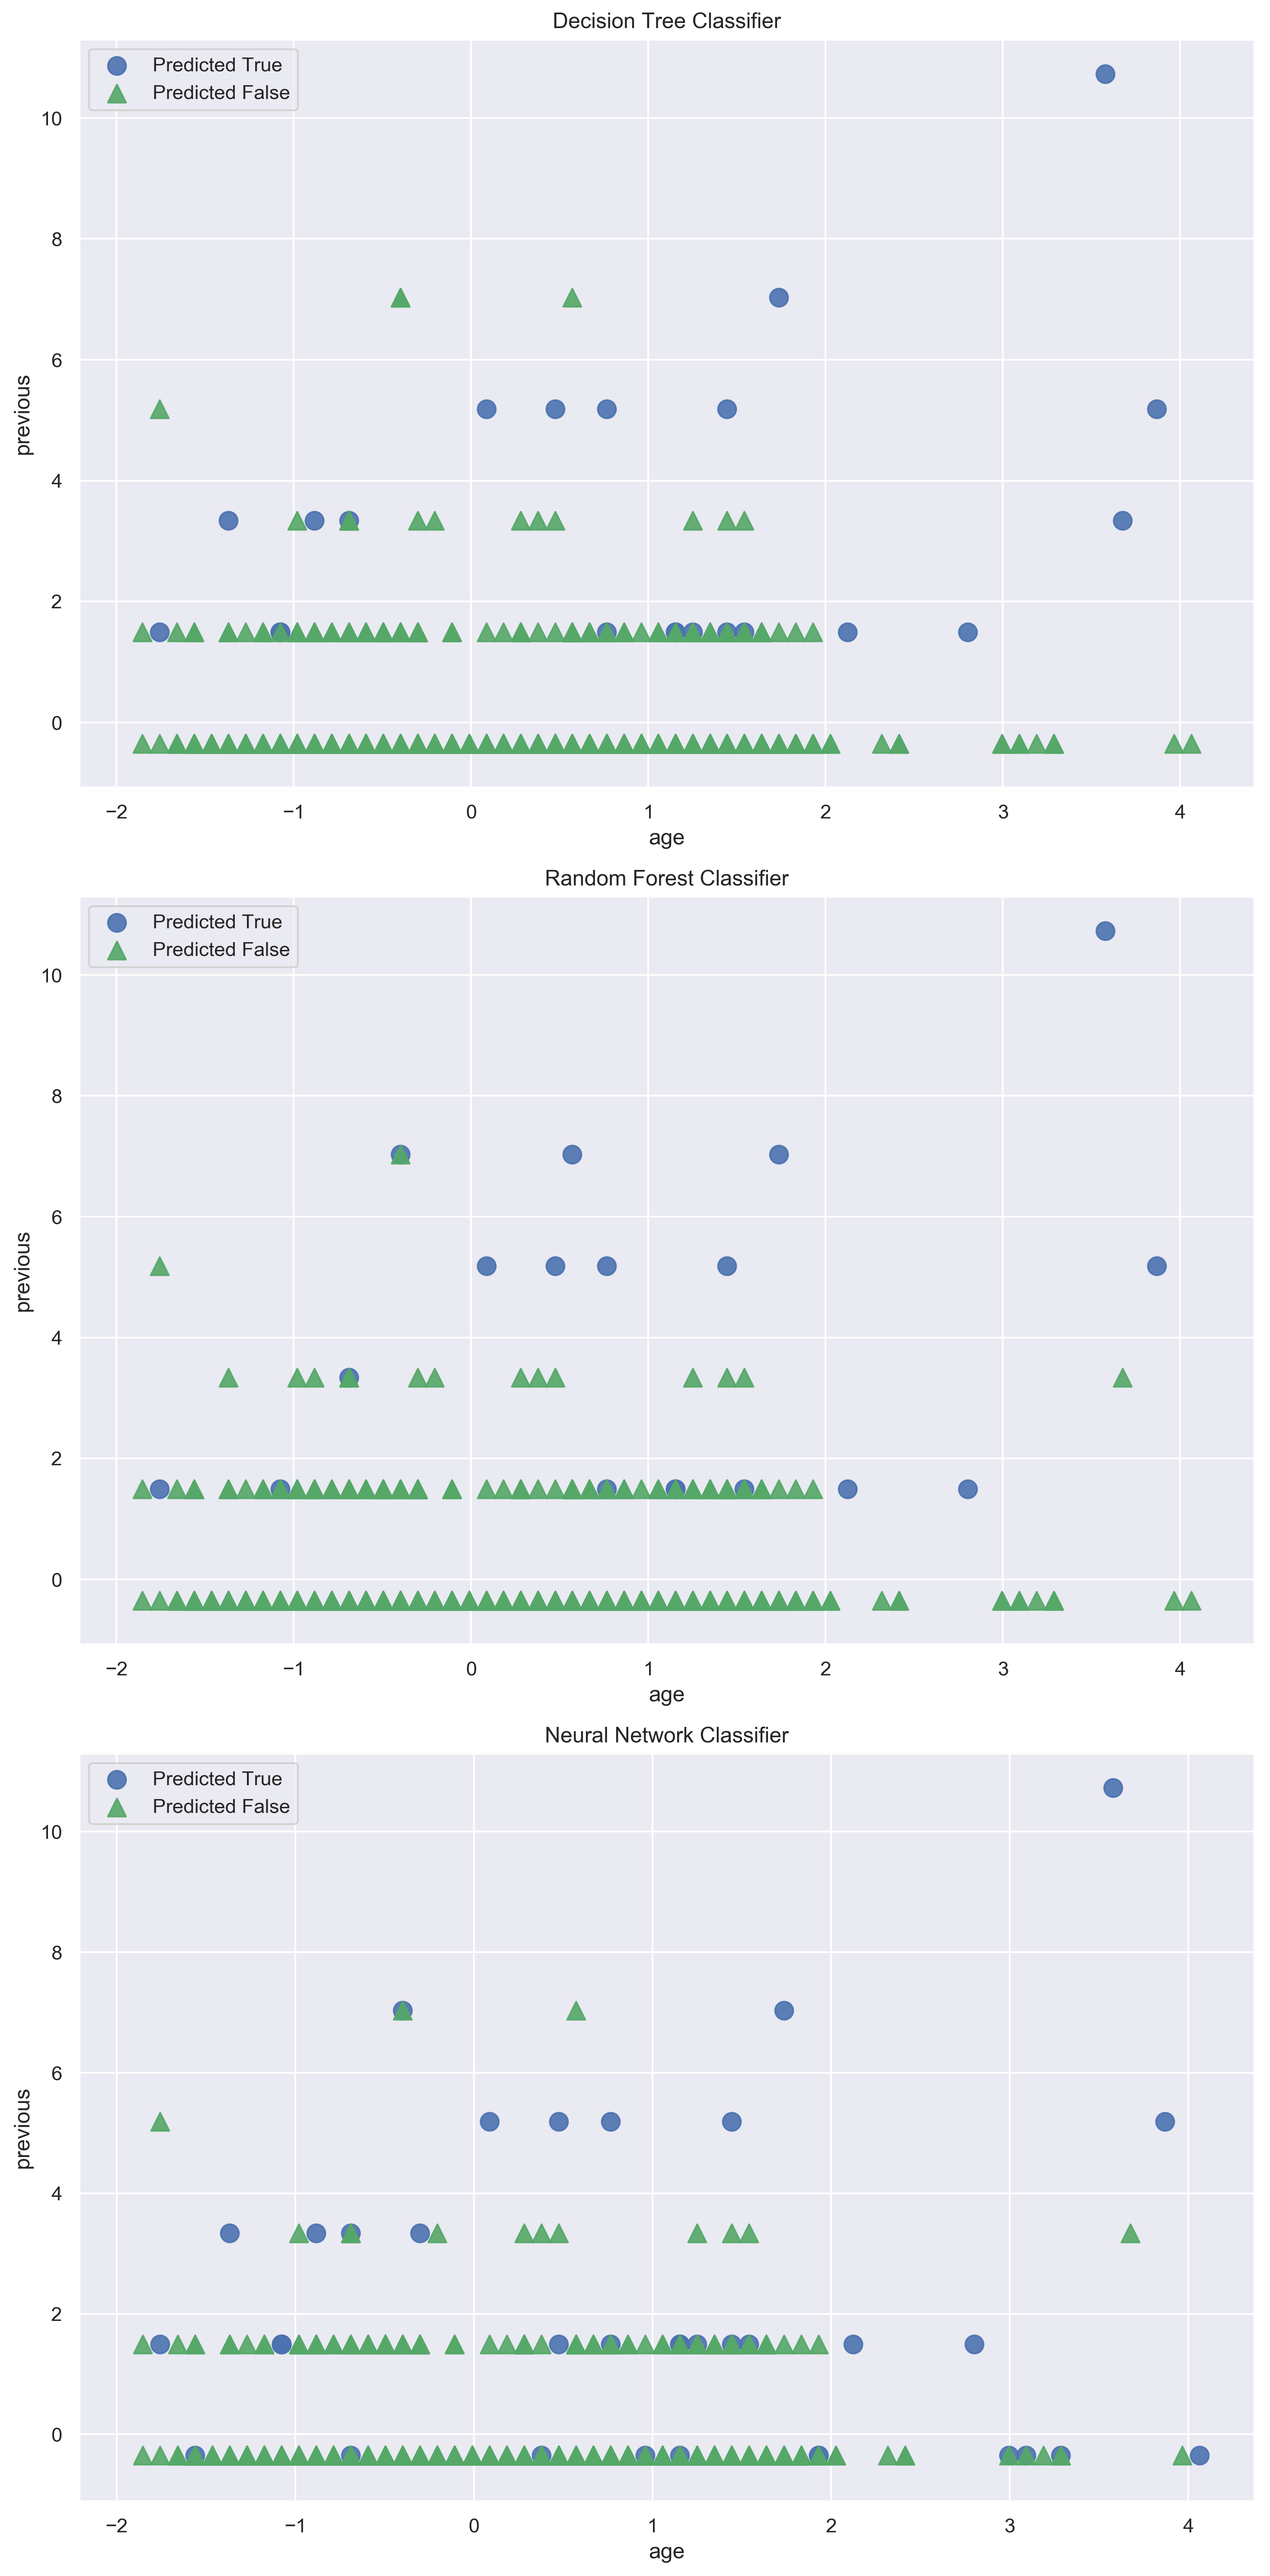
\includegraphics[width=2.5]{assignment2/1-4-age and previous features.png}
\caption{\label{fig:2dplot1}Plot of age VS previous }
\end{figure}


\clearpage{}
\begin{figure}[!ht]
 \centering
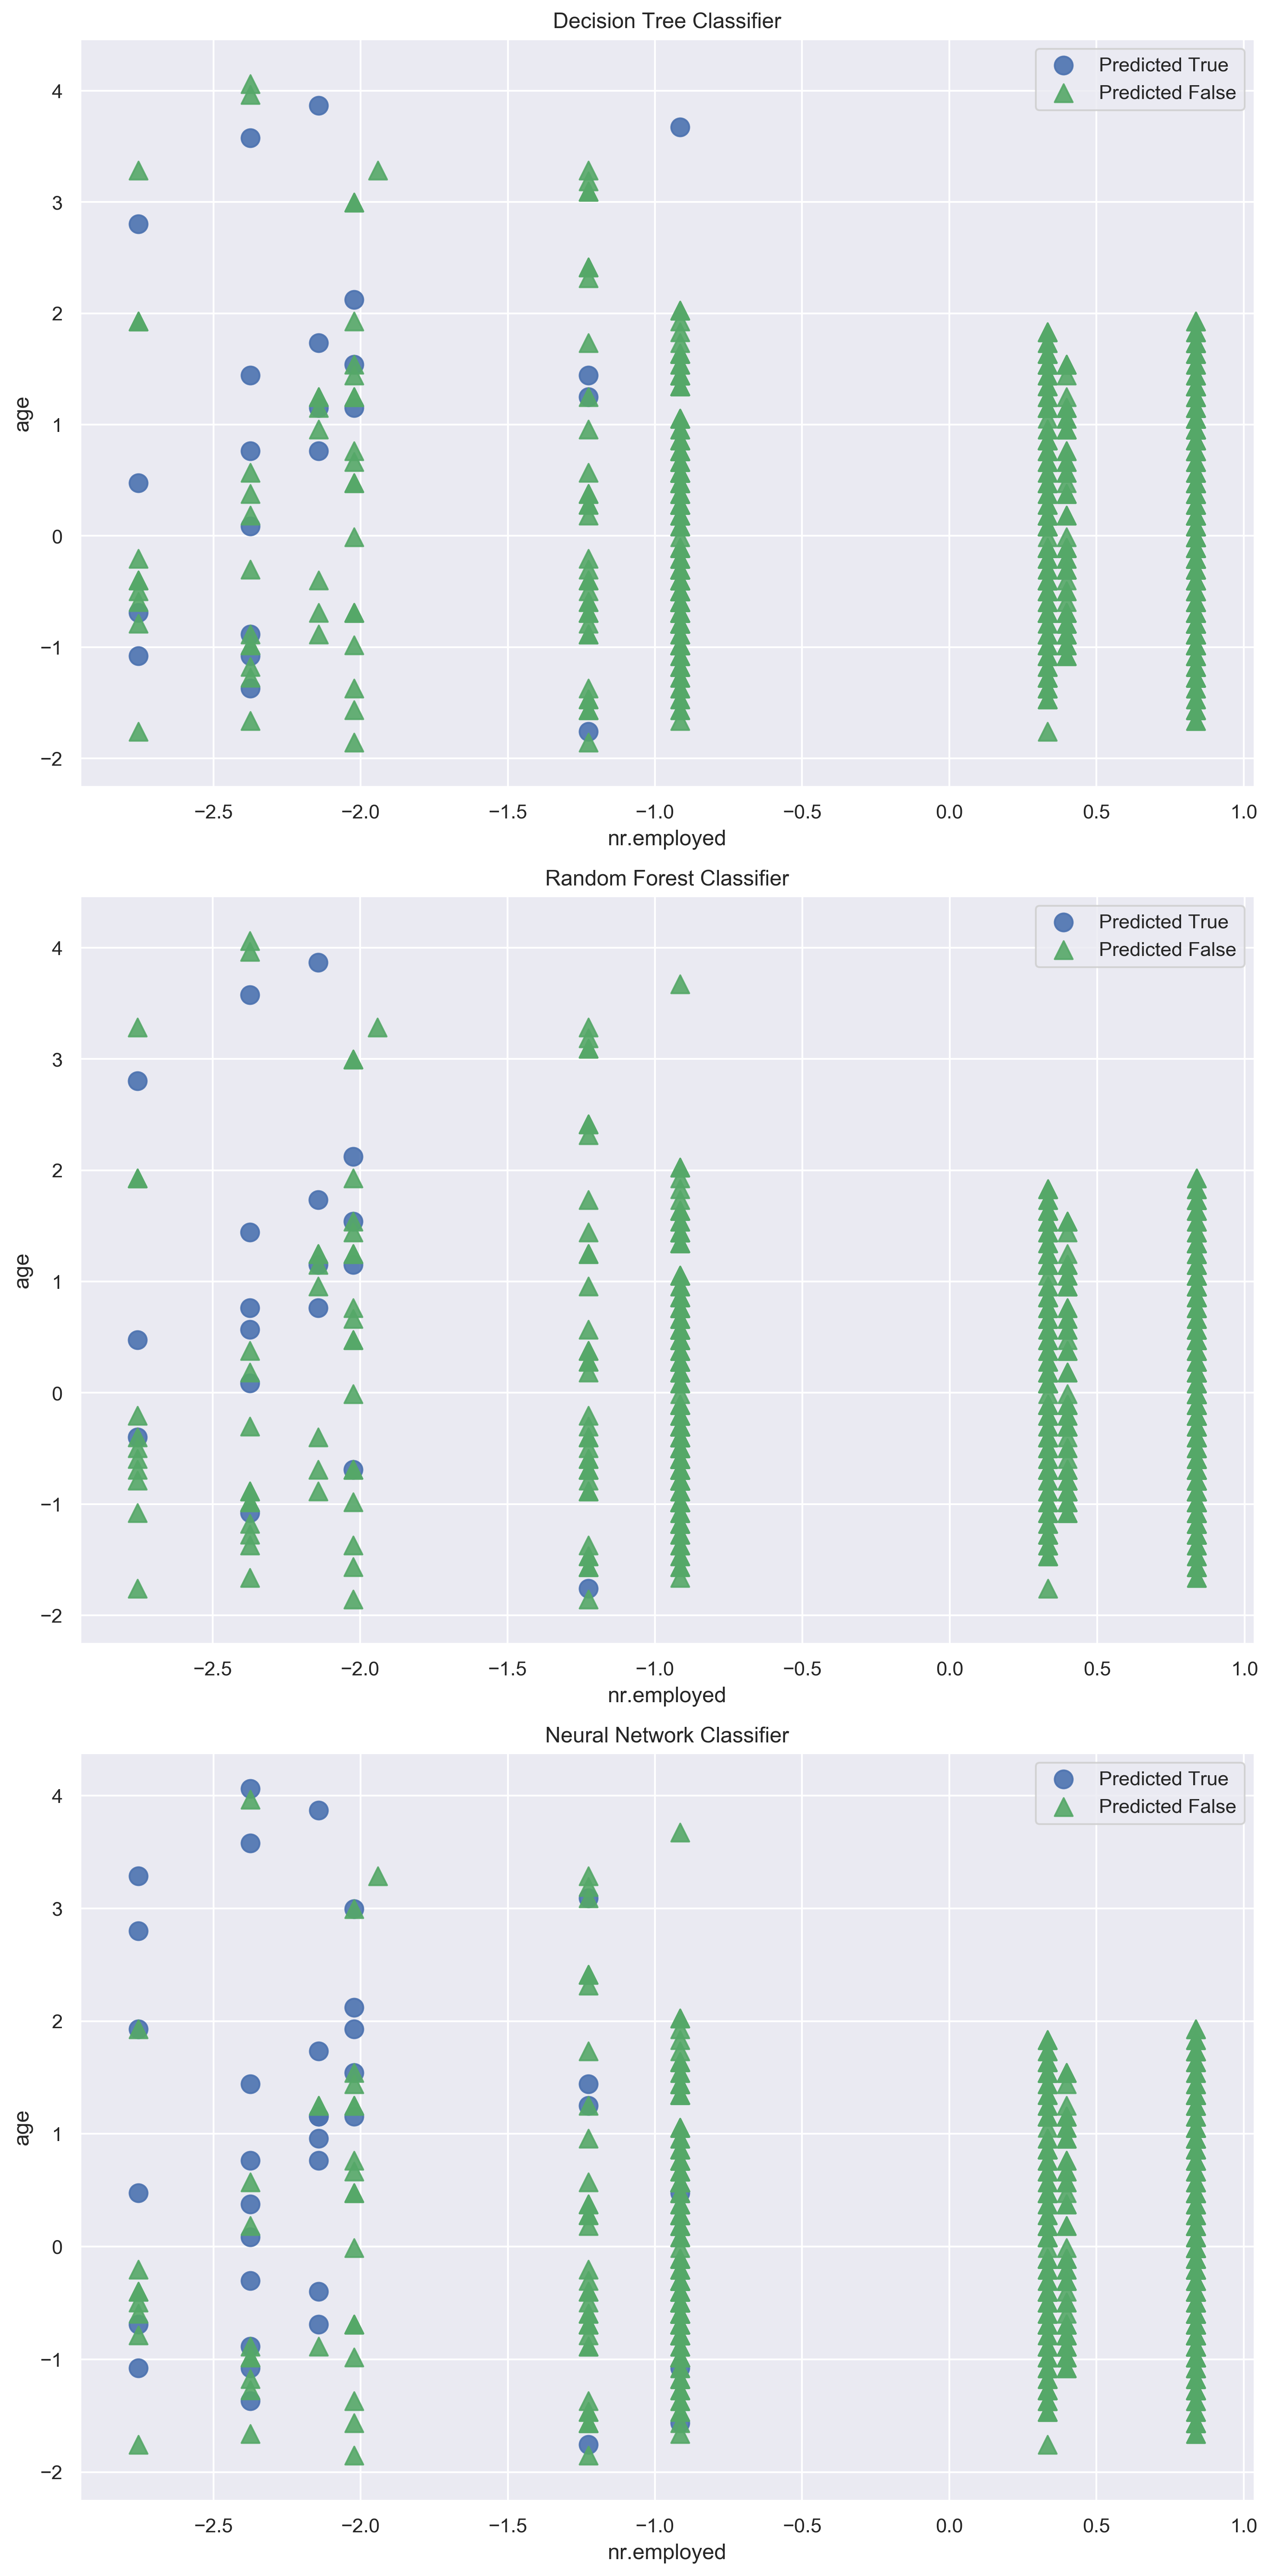
\includegraphics[width=2.5]{assignment2/1-4-age and nremployed features.png}
\caption{\label{fig:2dplot1}Plot of age VS nr.employed }
\end{figure}
\\


\newpage
\subsection{Produce a table with the true/false positive/negative metrics as well as accuracy's. Compare the values using bar charts}

Figure~\ref{fig:fig4} shows the comparison between true/false positive/negative metrics as well as accuracies. 
\begin{figure}[!ht]
 \centering
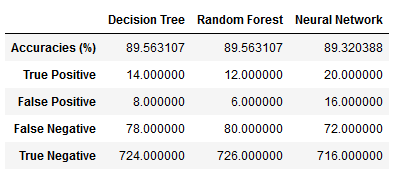
\includegraphics[width=3.0in]{assignment2/1-5_table.png}
\caption{\label{fig:fig4}table of metrics/accuracies and algorithms}
\end{figure}
\\
Figure~\ref{fig:fig5} shows the comparison between true/false positive/negative metrics as well as accuracies. We see from the bar charts that neural network performed better in classifying true positives and false negatives as compared to decision trees and random forests. However, decision tree and random forest had a higher values classifying false positive and true negative values. Comparing the overall accuracies, we see that all three models had almost similar accuracies (around 89\%).
\begin{figure}[!ht]
 \centering
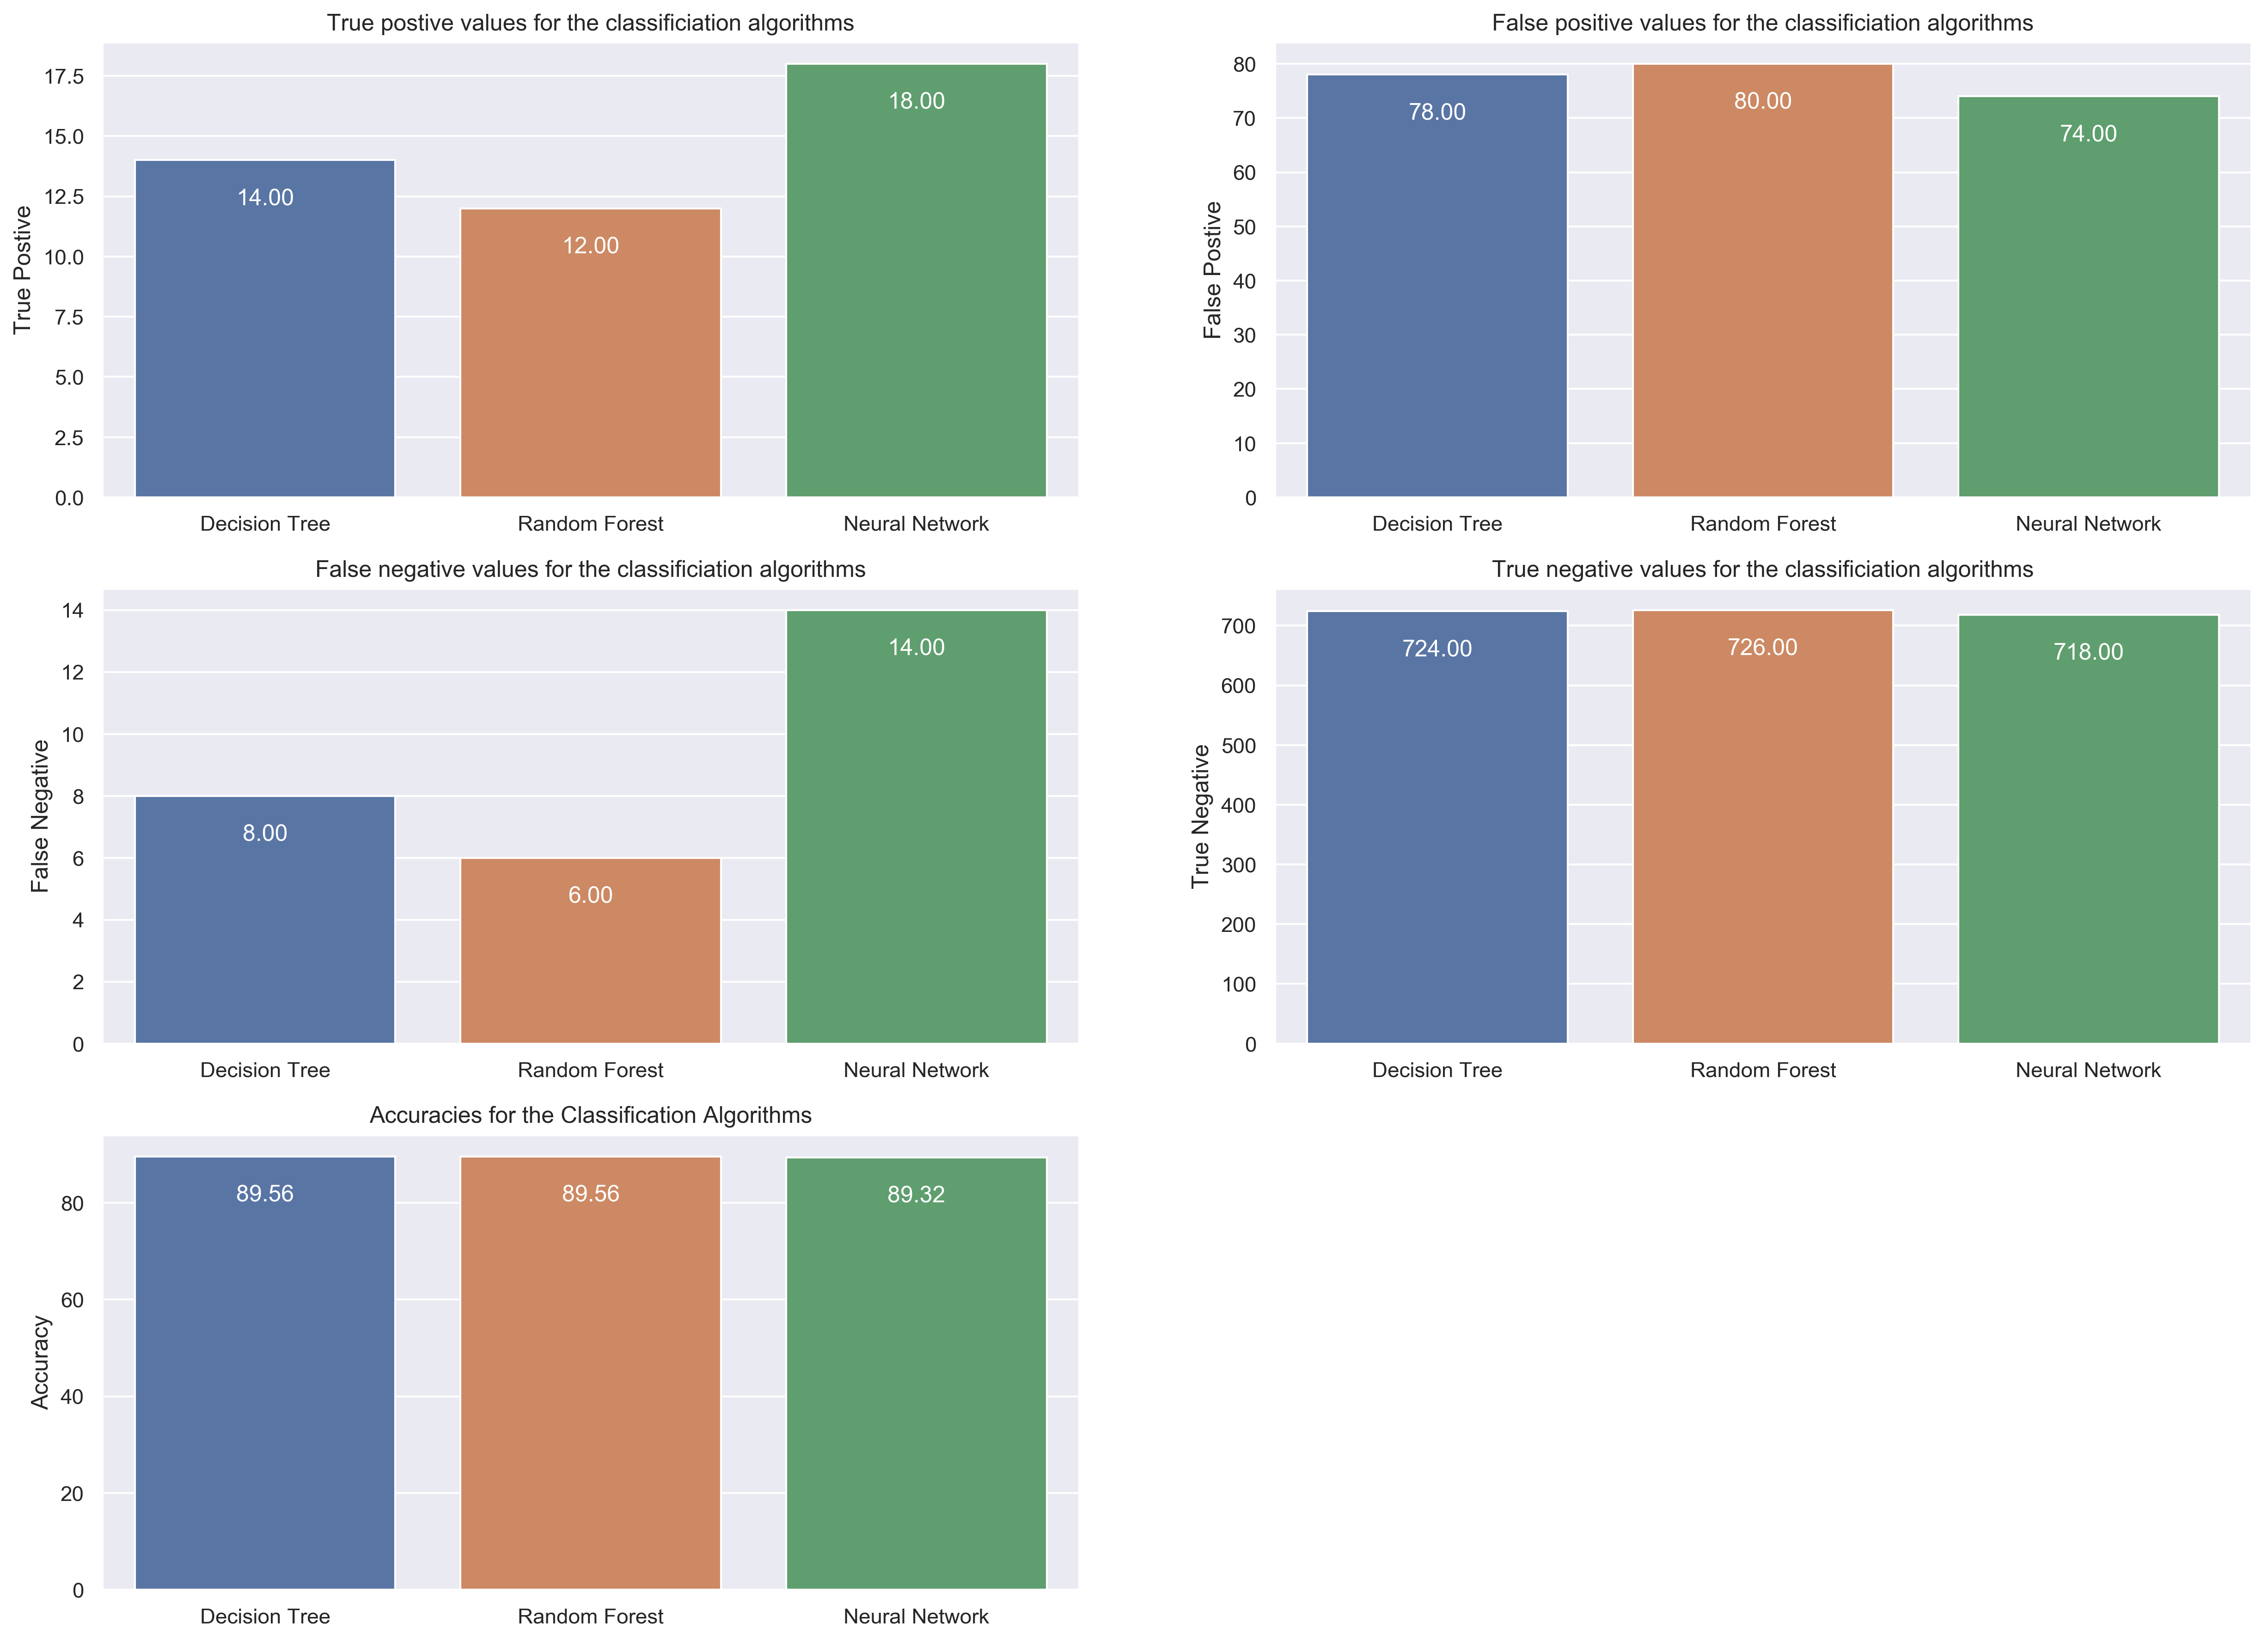
\includegraphics[width=5.1in]{assignment2/barcharts_algorithms.png}
\caption{\label{fig:fig5}bar charts of metrics/accuracies and algorithms}
\end{figure}

\\


\newpage
\subsection{Provide a short explanation of the results you have shown and what it means. Which classification method performed better? Why? Contrast performance with classification from the previous homework and comment on the difference, if any}
In this case ,if a customer will subscribe to term deposit at the bank is interpreted as "1"(Yes) and if a customer will not subscribe to term deposit is interpreted as "0"(No).\\
From the confusion matrix we get the True positive values  which represents the number of actual label (1's) predicted correctly as (1's) by our model and false positives(type 1 error) values represents the number of the  actual label (0's) predicted wrongly as (1's) by the model. True negative values represents the number of actual label (0's) predicted correctly as (0's) by our model. False negatives(type ii error) values represents the number of the  actual label (1's) predicted wrongly as (0's) by the model, here the model fails to detect an effect. Based on the bar chart above, we see that the neural network performed better at predicting the true positives compared to decision tress and random forests. Neural network also had the least miss-classification of the false positives. 



\subsection{Bonus: attempt at least one method to tackle the discrepancy in the size of the classes (imbalanced data)}
There are several methods to handle imbalanced data\cite{ref_url2}\\
1- Up-sample Minority Class(attempted)\\
2- Down-sample Majority Class(attempted)\\
3- Change Your Performance Metric(attempted)\\
4- Penalize Algorithms (Cost-Sensitive Training)\\
5- Use Tree-Based Algorithms\\
Change your Performance Metric :
 I think to tackle the issue of imbalanced data,precision  recall curve should be used when analyzing each algorithms performance  .As we know , ROC/AUC uses TPR(True positive rate) on Y axis and FPR(False positive rate ) on X axis. So replacing the FPR with precision on the X axis of the AUC graph might be the way to go.
 Precision=(TP/TP +FP) FPR= (FP/TN+FP)
 Since there were lots of samples that were Negatives(No's) relative to the number of Positives(Yes's) samples, then precision might be more useful than false positive rate . This is because precision does not include the number of True Negatives in its calculation, and is not affected by imbalance.\\
 \newline
Up-sample Minority Class:
The new data has more observations than the original, and the ratio of the two classes is now 1:1.(3668 observations for both classes).\\
It is clear that accuracy increased compared to our previous results.This result makes more sense and is a better performance metric
\begin{figure}[!ht]
 \centering
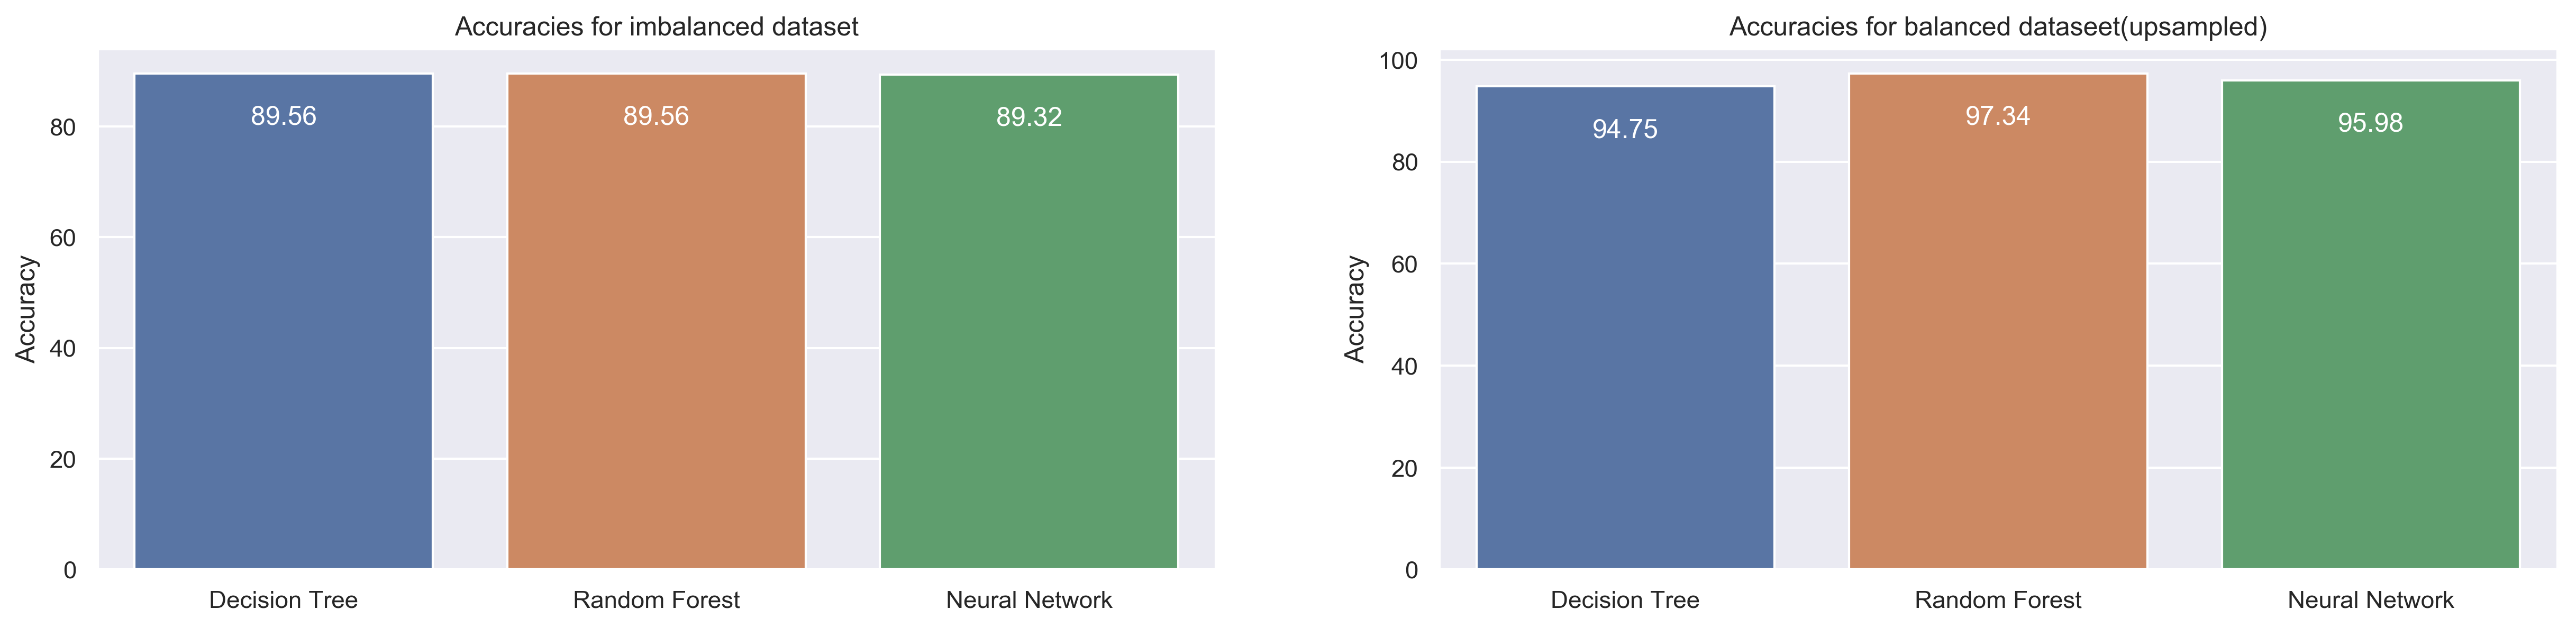
\includegraphics[width=6.1in]{assignment2/1-7-barcharts_up.png}
\caption{\label{fig:fig5}Accuracies after Upsampling }
\end{figure}
\newline
Down-sample Majority:
The new data has less observations than the original, and the ratio of the two classes is now 1:1.(451 observations for both classes).\\
It is clear that accuracy decreased compared to our previous results. This may be because we decreased the size of our data dramatically.
\begin{figure}[!ht]
 \centering
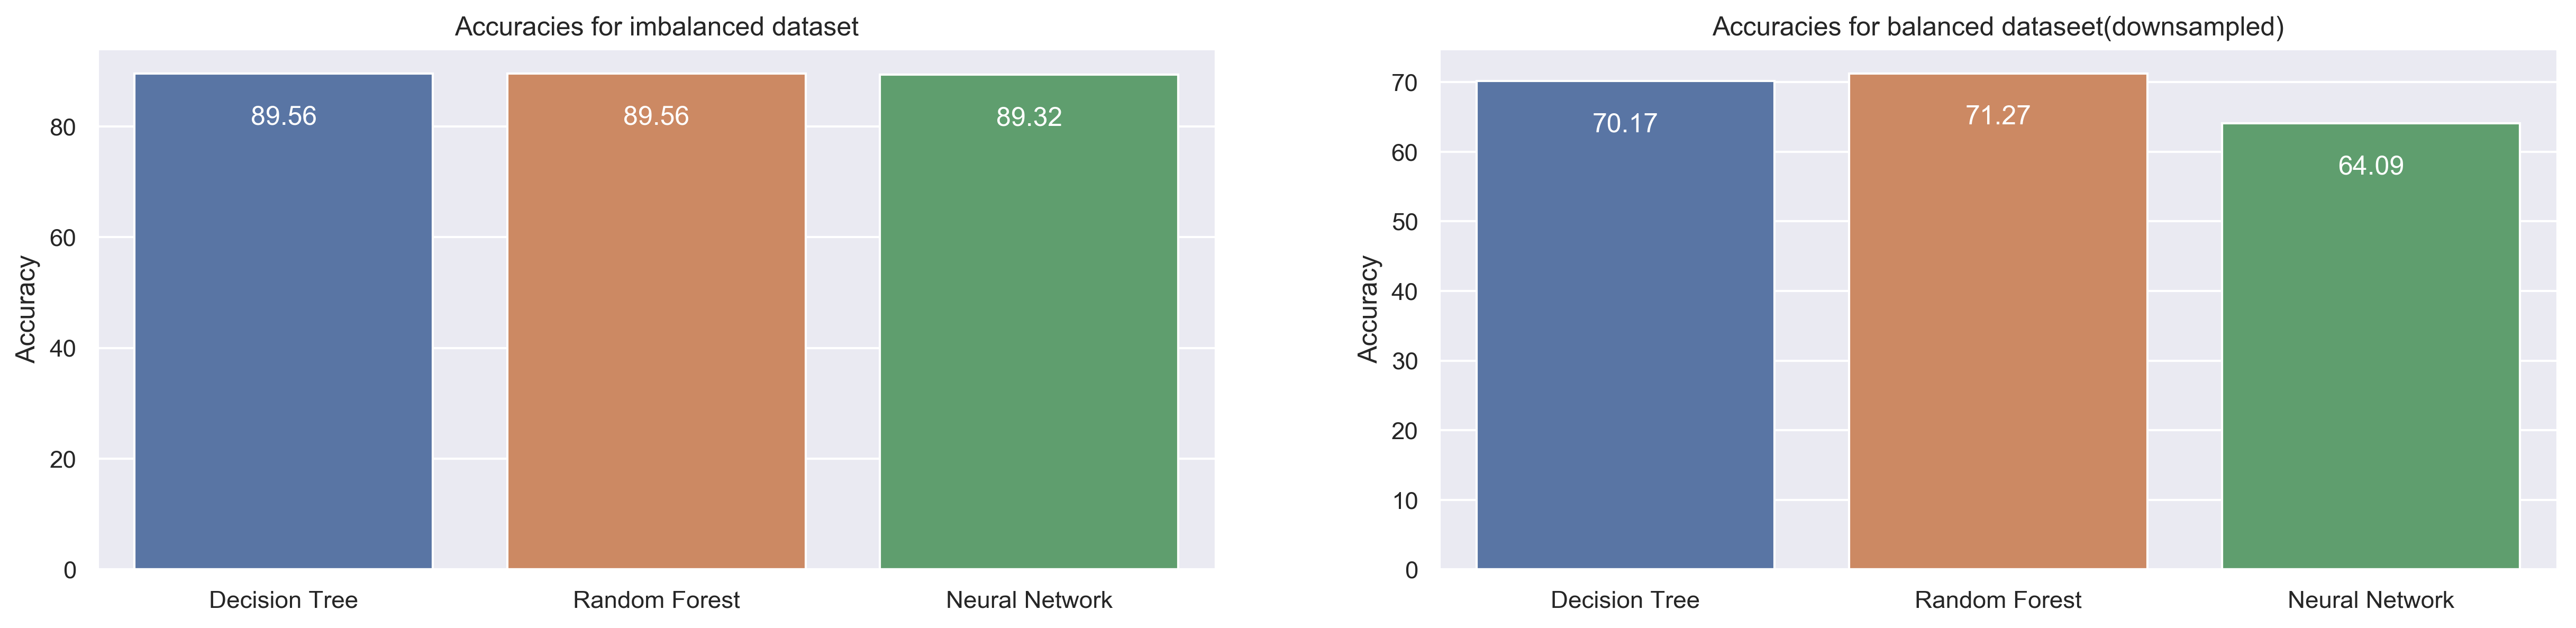
\includegraphics[width=6.1in]{assignment2/1-7-barcharts_dn.png}
\caption{\label{fig:fig5}Accuracies after Downsampling }
\end{figure}



